\documentclass[a4paper, 12pt]{ctexart}
\usepackage[UTF8]{ctex}
\usepackage{graphicx}
\usepackage{grffile}
\usepackage{longtable}
\usepackage{wrapfig}
\usepackage{rotating}
\usepackage{amsmath}
\usepackage{mathrsfs}
\usepackage{amssymb} 
\usepackage{amsmath} 
\usepackage{amsthm}
\usepackage{xltxtra} 
\usepackage{mflogo,texnames}
\usepackage{indentfirst}
\usepackage[normalem]{ulem}
\usepackage{textcomp}
\usepackage{booktabs}
\usepackage[linktocpage,pdfstartview=FitH,colorlinks,
linkcolor=blue,anchorcolor=blue,
citecolor=blue,filecolor=blue,menucolor=blue,urlcolor=blue]{hyperref}
\usepackage{setspace,csquotes, enumitem,endnotes,fontspec, capt-of}
\doublespacing
\usepackage[margin=1in]{geometry}
\usepackage[notes, notetype=endonly, isbn=false, backend=biber]{biblatex-chicago}
\bibliography{shiff2016b}
\let\footnote=\endnote
\let\cite=\endnote
\let\footcite=\autocite
\setCJKmainfont{SimSun}
\CTEXsetup[format={\Large\bfseries}]{section}
\setlist[enumerate,itemize]{noitemsep,nolistsep,leftmargin=*}
\newtheorem*{theorem}{定理}
\newtheorem*{example}{例子}


\author{张天骏 \\ 2021300003004}
\date{}
\title{跳过程介绍}


\begin{document}
\maketitle

\newpage
\tableofcontents   

\section*{}
\section*{}
\begin{figure}[hb]
    \centering
    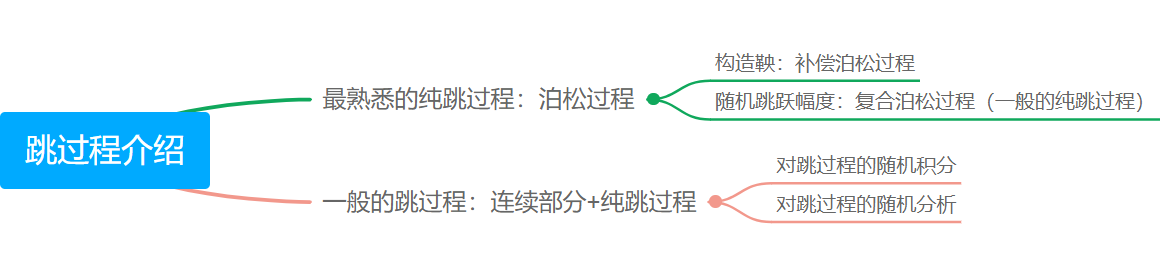
\includegraphics[width=0.8\linewidth]{pic/大纲.png}
    \nonumber
    \label{fig:enter-label}
\end{figure}


\newpage
\section{泊松过程$N(t)$}
\begin{figure}[h]
    \centering
    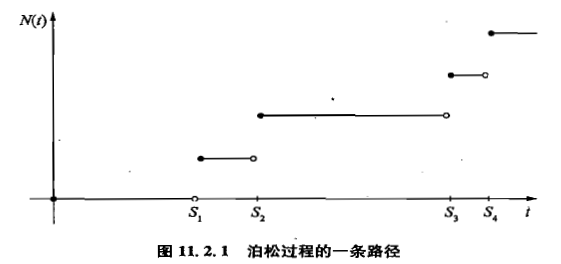
\includegraphics[width=0.8\linewidth]{pic/泊松.png}
    \nonumber
    \label{fig:enter-label}
\end{figure}
考虑独立增量的计数过程$N(t) \in \{ 1,2,\cdots n \cdots\}$,记$S_n$为第$n$次跳跃的时间,$\lambda$为跳跃的平均等待时间。
则泊松过程$N(t)$定义为:
$$N(t)=\begin{cases} 0,0 \leq t \leq S_1\\ 1,S_1 \leq t \leq S_2 \\ 2,S_2 \leq t \leq S_3 \\ \ \vdots \end{cases}$$

\begin{theorem}
     $N(t)$服从强度为$\lambda$的泊松分布;
     $S_1 \text{:第1次跳跃等待时间}$服从强度为$\lambda$的指数分布;
     $S_n \text{:前n次跳跃用时}$服从$\Gamma(n,\lambda)$分布
\end{theorem}

\subsection{补偿泊松过程$M(t)$}
\begin{figure}[h]
    \centering
    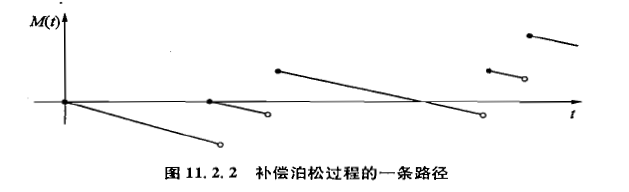
\includegraphics[width=0.8\linewidth]{pic/补偿.png}
    \nonumber
    \label{fig:enter-label}
\end{figure}

由于泊松过程是一个增过程,所以们考虑它的$\text{Doob-Meyer}$分解,$M(t)=N(t)-E(N(t))=N(t)-\lambda t$,
很容易证明$M(t)$是一个鞅:
\begin{proof}
    给定$0\leqslant t\leqslant s$,由于 $N(t)-N(s)$独立于 $F(s)$,并且具有期望值$\lambda (t-s)$,我们有:
    \begin{align*}
        E[M(t)|F(s)]=&E[M(t)-M(s)|F(s)]+E[M(s)|F(s)] \\
        =&E[N(t)-N(s)-λ(t-s)|F(s)]+M(s) \\
        =&E[N(t)-N(s)]-λ(t-s)+M(s) \\
        =&M(s)
    \end{align*}
\end{proof}


\subsection{复合泊松过程$Q(t)$}
\begin{figure}[h]
    \centering
    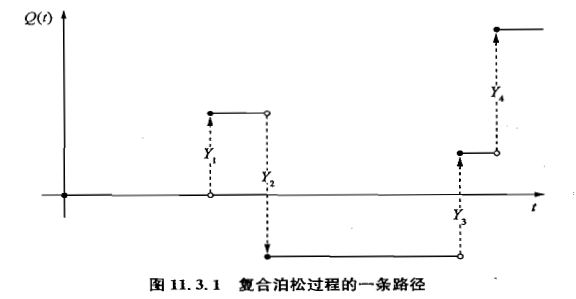
\includegraphics[width=0.8\linewidth]{pic/复合.png}
    \nonumber
    \label{fig:enter-label}
\end{figure}

基于泊松过程构造复合泊松过程:

\begin{itemize}
    \item 设 $N(t)$是强度为$\lambda$的泊松过程,$Y_1 ,Y_2 \dots$是一列均值为$\beta$的同分布随机变量。假设随机变量$Y_1 ,Y_2 \dots$两两独立,并且也独立于泊松过程 $N(t)$ 
    \item 定义复合泊松过程  $Q(t)=\sum_{i=1}^{N(t)}Y_i,t \geqslant 0$ 
    \item $Q(t)$与$N(t)$在同一时刻发生跳跃,$N(t)$的跳跃幅度恒为 1,而 $Q(t)$的跳跃幅度则随机。第一次跳跃幅度为$Y_1$,第二次跳跃幅度为$Y_2$……
    \item 类似的,$Q(t)$也有补偿过程(取$\text{Doob-Meyer}$分解即可)
\end{itemize}

下面我们计算复合泊松过程$Q(t)$的矩母函数:
\begin{align*}
    \phi(u) &= \mathbb{E}e^{uQ(t)} = \mathbb{E}e^{u\sum_{i=1}^{N(t)}Y_i} \\ 
    &= \mathbb{P}{N(t) = 0} + \sum_{k=1}^{\infty} \mathbb{E}\left[e^{u\sum_{i=1}^k Y_i} \Big| N(t) = k\right]\mathbb{P}\{N(t) = k\} \\ 
    &= \mathbb{P}{N(t) = 0} + \sum_{k=1}^{\infty} \mathbb{E}\left[e^{u\sum_{i=1}^k Y_i}\right]\mathbb{P}\{N(t) = k\} \\ 
    &= e^{-\lambda t} + \sum_{k=1}^{\infty} \mathbb{E}e^{uY_1} \mathbb{E}e^{uY_2} \cdots \mathbb{E}e^{uY_k} \frac{(\lambda t)^k}{k!} e^{-\lambda t} \\ 
    &= e^{-\lambda t} + e^{-\lambda t} \sum_{k=1}^{\infty} \left(\phi_Y(u)\lambda t\right)^k \frac{1}{k!} \\
    & = \sum_{k=0}^{\infty} \left(\phi_Y(u)\lambda t\right)^k \frac{1}{k!} \\
    & = \exp \left(\lambda t (\phi_{Y}(u)-1)\right)
\end{align*}

\begin{itemize}
    \item 如果$Y_{i}=y$:$\phi(u)=\exp(\lambda t(e^{  uy}-1))$
    \item 如果$Y_{i}=1$:$\phi_{Poisson}(u)=\exp(\lambda t(e^{  u}-1))$
    \item 如果$Y_{i}$只取有限多个值:$\phi_{Y}(u)=\mathbb{E}\exp(uy)=\sum_{m=1}^M \mathbb{P}_{y_{m}} \exp(uy_{m})$,
          从而:
            \begin{align*}
                \phi(u)&=\exp \left[ \lambda t\left( \sum_{m=1}^M \mathbb{P}_{y_{m}} \exp(uy_{m})-1 \right) \right] \\
                &=\prod_{m=1}^M  \exp[\lambda \mathbb{P}_{y_{m}}t(e^{uy_{m}}-1)] 
            \end{align*}
\end{itemize}



\subsection{分解定理}
\begin{theorem}
    设$y_{1},y_{2} \dots,y_{M}$是非零常数的有限集,$\rho(y_{1}) \rho(y_{2}) \cdots \rho(y_{M})$是总和为1的正数。
给定$\lambda>0$,设$\overline{N}_{1}(t) \overline{N}_{2}(t) \cdots\overline{N}_{M}(t)$是两两独立的泊松过程,
每个$\overline{N}_{m}(t)$具有强度$\lambda\rho(y_{m})$.定义:
$$Q(t) = \sum_{m=1}^{M} y_{m}\overline{N}_{m}(t),\quad t\geqslant0$$
则$\overline{Q}(t)$是复合泊松过程。如果$\overline{Y}_{1}$是$\overline{Q}(t)$的第一次跳跃的幅度,$\overline{Y}_{2}$是$\overline{Q}(t)$
的第二 次跳跃的幅度,等等,并且
$$\overline{N}(t)=\sum_{m=1}^{M}\overline{N}_{m}(t),\quad t\geqslant0$$
是时间区间$(0,t]$内的跳跃总数,
则$\overline{N}(t)$是强度为$\lambda$的泊松过程,随机变量$\overline{Y}_{1},\overline{Y}_{2}$,…两两独立,
$\mathbb{P}({\overline{Y_i} = y_m})=p (\overline{y_{m}}),m=1\cdots,M,$随机变量$\overline{Y}_{1},…,\overline{Y}_{M}$独立于$\overline{N}(t)$,并且
$$\overline{Q(t)}= \sum_{i=1} ^{\overline{N}(t)}\overline{Y}_{i},\quad t\geqslant0$$
\end{theorem}

\begin{proof}
    由级数换序
    $$Q(t)=\sum_{i=1}^{N(t)}Y_{i}=\sum_{m=1}^M y_{m}N_{m}(t)=\sum_{i=1}^{N(t)} \sum_{m=1}^M Y_{i}\mathbb{1}_{Y_{i}=y_m}$$
    可以得到二者的等价性
\end{proof}

\section{一般的跳过程}
$$X(t)=\underset{initial}{X(0)}+\underset{ It\ddot{o} }{ I(t) }+\underset{ Riemann }{ R(t) }+\underset{ Jump }{ J(t) }$$


\begin{itemize}
    \item $I(t) = \int_0^t \Gamma(s)dW(s)$
    \item $R(t) = \int_0^t \Theta(s)ds$
    \item 定义该过程的连续部分$X^c(t)=X(0)+I(t)+R(t)=X(0)+\int_0^t \Gamma(s)dW(s)+ \int_0^t \Theta(s)ds$
    \begin{itemize}
        \item $[X^c(t),X^c(t)]=\int_0^t \Gamma^{2}(s)ds$
    \end{itemize}
    \item $J(t)$是纯跳过程:右连续、两次跳跃之间是常数、假设有限时间内跳跃有限多次
    \begin{itemize}
        \item 纯跳过程的左连续形式记作$J(t-):=\lim_{ s \to t^- }J(t)$  对应着跳跃之前的瞬间
        \item 纯跳过程$t$时刻的跳跃幅度记作$\Delta J(t):=J(t)-J(t-)$
    \end{itemize}
\end{itemize}


\section{跳过程的随机积分}
$\int_0^t \Phi(s)dX(s) = \int_0^t \Phi(s)\Gamma(s)dW(s) + \int_0^t \Phi(s)\Theta(s)ds+ \underset{ 0<s\leq t }{ \sum }\Phi(s)\Delta I(s)$

它对应的微分形式如下:
\begin{align*} \Phi(t)dX(t) &= \Phi(t)dI(t) + \Phi(t)dR(t) + \Phi(t)dJ(t)\\ &= \Phi(t)dX^c(t)+ \Phi(t)dJ(t)\\
    &=\Phi(t)\Gamma(t)dW(t) + \Phi(t)\Theta(t)dt+ \Phi(t)dJ(t)
\end{align*}

    

\subsection{鞅性}
我们在关于连续过程(比如说布朗运动)的积分时曾提及“适应过程关于一个鞅过程的随机积分是鞅”,
在这里还成立吗?我们可以举出一个反例。

\begin{example}
关于$X(t)=M(t)=N(t)-\lambda t$ 补偿泊松过程的积分  被积式是$\Delta N(t)$ 定义同上
\begin{itemize}
    \item $\int_0^t\Phi(s)dX^c(s)=\int_0^t\Phi(s)dR(s)=-{\lambda}\int_0^td\Phi(s)=0$
    \item $\int_0^t\Phi(s)\mathrm{d}N(s)=\sum_{0<s\leqslant t}(\Delta N(s))^2=N(t)$
    \item $\int_0^t\Phi(s)\mathrm{d}M(s)=-\lambda\int_0^t\Phi(s)\mathrm{ds}+\int_0^t\Phi(s)\mathrm{d}N(s)=N(t)$
\end{itemize}

此时$\mathbb{E}(\int_0^t\Phi(s)\mathrm{d}M(s)|M(t'))=\mathbb{E}(N(t)|M(t'))=\lambda(t-t')\neq 0$ 由此可以看出,适应过程关于跳鞅的随机积分不一定是鞅。
\end{example}

那么我们需要加强什么条件才能得到跳过程随机积分的鞅性?我们有如下定理

\begin{theorem}
    如果被积过程是左连续、$\mathscr{L}^2$可积、适应过程。那么跳过程关于该过程的随机积分是鞅。
    (这个条件可以减弱为可料过程)
\end{theorem}

\subsection{二次变差和交互变差}
\begin{theorem}
    给定两个跳过程$X_1 (t),X_2 (t)$,我们可以计算出它们各自的二次变差和交互变差:

$[X_{1},X_{1}]^{}(T)=[X_{1}^{c},X_{1}^{c}]^{}(T)+[J_{1},J_{1}]^{}(T)=\int_{0}^{T}\Gamma_{i}^{2}(s)ds+\underset{{0<s\leq T}}{\sum}(\Delta J_{1}(s))^{2}$

$[X_1, X_2](T) = [X_1^c, X_2^c](T) + [J_1, J_2](T)= \int_0^T \Gamma_1(s)\Gamma_2(s)ds + \underset{{0<s\leq T}}{\sum}\Delta J_1(s)\Delta J_2(s)$

\end{theorem}

由于二次变差是交互变差的特例,我们在这里只证明交互变差的式子:
\begin{proof}
    \begin{align*} c_{\prod}(X_1,X_2) &= \sum_{i=0}^{n-1}(X_1(t_{i+1}) - X_1(t_i))(X_2(t_{i+1}) - X_2(t_i))\\ 
        &= \sum_{i=0}^{n-1}(X_1 ^c(t_{i+1}) - X_1  ^c(t_i) + J_1(t_{i+1}) - J_1(t_i))\times(X_2 ^c(t_{i+1}) - X_2 ^c(t_i) + J_2(t_{i+1}) - J_2(t_i))\\ 
        &= \sum_{i=0}^{n-1}(X_1 ^c(t_{i+1}) - X_1 ^c(t_i))(X_2(t_{i+1}) - X_2 ^c(t_i))+ \sum_{i=0}^{n-1}(X_1 ^c(t_{i+1}) - X_1 ^c(t_i))(J_2(t_{i+1}) - J_2(t_i))\\ 
        &\quad+ \sum_{i=0}^{n-1}(J_1(t_{i+1}) - J_1(t_i))(X_2 ^c(t_{i+1}) - X_2 ^c(t_i))+ \sum_{i=0}^{n-1}(J_1(t_{i+1}) - J_1(t_i))(J_2(t_{i+1}) - J_2(t_i)) 
    \end{align*}
    
    其中:
    \begin{align*}
        &\left|\sum_{j=0}^{n-1}\left(X_{1}^{c}(t_{j+1})-X_{1}^{c}(t_{j})\right)\left(J_{2}(t_{j+1})-J_{2}(t_{j})\right)\right|  \\
        &\leqslant\max_{0\leqslant j\leqslant n-1}\left|(X_{1}^{c}(t_{j+1})-X_{1}^{c}(t_{j}))\right|\cdot\sum_{j=0}^{n-1}\left|(J_{2}(t_{j+1})-J_{2}(t_{j})\right| \\
        &\leqslant\max_{0\leqslant j\leqslant n-1}\left|(X_{1}^{c}(t_{j+1})-X_{1}^{c}(t_{j}))\right|\cdot\sum_{0\leqslant s\leqslant T}\left|\Delta J_{2}(s)\right| ;
        \\ 
        & \sum_{j=0}^{n-1}\left(J_1\left(t_{j+1}\right)-J_1\left(t_j\right)\right)\left(J_2\left(t_{j+1}\right)-J_2\left(t_j\right)\right) \\
        & =\sum_{j \in A_1 \cap A_2}\left(J_1\left(t_{j+1}\right)-J_1\left(t_j\right)\right)\left(J_2\left(t_{j+1}\right)-J_2\left(t_j\right)\right) \\
        & = \sum_{0<s\leq t}\Delta J_1(s)\Delta J_2(s)
        \end{align*}
    带入可以得到:$$c_{\prod}(X_1,X_2)=\sum_{i=0}^{n-1}(X_1 ^c(t_{i+1}) - X_1 ^c(t_i))(X_2 ^c(t_{i+1}) - X_2 ^c(t_i))+\sum_{i=0}^{n-1}(J_1(t_{i+1}) - J_1(t_i))(J_2(t_{i+1}) - J_2(t_i))$$
    令$n \to \infty$:$$[X_1, X_2](T) = [X_1^c, X_2^c](T) + [J_1, J_2](T)= \int_0^T \Gamma_1(s)\Gamma_2(s)ds + \underset{{0<s\leq T}}{\sum}\Delta J_1(s)\Delta J_2(s) $$ 
\end{proof}

由证明过程我们可以发现:一个跳过程可以分解为“正交”的两部分:连续部分+纯跳部分

\section{跳过程的$I\ddot{t}o$公式}
\begin{theorem}
    跳过程的$I\ddot{t}o$公式如下:
$$\begin{small}
    f(X(t)) =f(X(0))+\int_0^tf'(X(s))dX^c(s)+\frac{1}{2}\int_0^tf''(X(s))dX^c(s)dX^c(s)+\underset{{0<s\leq T}}{\sum}f(X(s))-f(X(s-))
\end{small}$$
\end{theorem}

\begin{proof}
    若时域$[u,v]$没有发生跳跃,则$X(t)$的$I\ddot{t}o$公式为:

    $f(X(t)) =f(X(0))+\int_0^tf'(X(s))dX^c(s)+\frac{1}{2}\int_0^tf''(X(s))dX^c(s)dX^c(s)$

    此时对于时域$[0,t]$,沿着跳时刻${\tau_{i}}$切分($n$维情景就进一步切分为$\cup_{n}\{ \tau^n_{i}\}$)
    只要保证积分区间(时域)没有跳,是连续的就行。这时仍有:
    $$f(X(\tau _{i+1}-))-f(X(\tau _{j}))=\int_{\tau _{j}}^{\tau _{i+1}}f^{\prime }(X(s))dX^{c}(s)+\frac{1}{2}\int_{\tau _{j}}^{\tau _{i+1}}f^{\prime \prime }(X(s))dX^{c}(s)dX^{c}(s)$$
    
    由$f(X(\tau _{i+1}))-f(X(\tau _{j}))  =f(X(\tau _{i+1}))-f(X(\tau _{i+1}-))+f(X(\tau _{i+1}-))-f(X(\tau _{j}))$可得:
    \begin{align*}
        f(X(\tau _{i+1}))-f(X(\tau _{j}))  =&\int_{\tau _{j}}^{\tau _{i+1}}f^{\prime }(X(s))ds+\frac{1}{2}\int_{\tau _{j}}^{\tau _{i+1}}f^{\prime \prime }(X(s))dX^{c}(s)dX^{c}(s) \\[0.5mm]
    &+f(X(\tau _{i+1})) -f(X(\tau _{i+1}-)) \end{align*}

    最后由$f(X(t))-f(X(0))=\underset{ i=1 }{ \overset{ n }{ \sum } } f(X(\tau _{i+1}))-f(X(\tau _{j}))$
    得到跳过程的$I\ddot{t}o$公式

\end{proof}

\subsection{例子:$It \ddot{o}$乘积法则}
给定两个跳过程$X_1 (t),X_2 (t)$,可以根据上文的$I\ddot{t}o$公式计算二者乘积过程的展开式:
\begin{align*}
    &X_1(t)X_2(t) \\
    =&X_1(0)X_2(0)+\int_0^tX_2(s)dX_1^c(s)+\int_0^tX_1(s)dX_2^c(s)+\left[X_1^c,X_2^c\right](t) \\
    &+\sum_{0<s\leq t}\left[X_1(s)X_2(s)-X_1(s-)X_2(s-)\right] \\
    =&X_1(0)X_2(0)+\int_0^tX_2(s-)dX_1(s)+\int_0^tX_1(s-)dX_2(s)+\left[X_1,X_2\right](t)
\end{align*}

至于两个式子的等价性,我们可以根据下面两个式子证明:
\begin{align*}
    &[X_{1},X_{2}](t)=[X_{1}^c,X_{2}^c](t)+[J_{1},J_{2}](t) \\
    &\sum_{0<s\leq t}\left[X_1(s)X_2(s)-X_1(s-)X_2(s-)\right]=\sum_{0<s\leq t}\left[X_1^c(s-)\Delta J_1(s)+X_2(s-)\Delta J_2(s)+\Delta J_1(s)\Delta J_2(s)\right]
\end{align*}


\subsection{例子:同一个域流下的布朗运动和泊松过程相互独立}
\begin{proof}
    我们考虑随机过程:$Y(t)=\exp\left\{u_1W(t)+u_2N(t)-\frac{1}{2}u_1^2t-\lambda(e^{u_2}-1)t\right\}$,其中
    $W(t)$是标准布朗运动,$N(t)$是泊松过程。
    
    如果该过程在$t=s$时发生跳跃,则:
    
    $Y(s)=\exp\left\{u_1W(s)+u_2\left(N(s-)+1\right)-\frac{1}{2}u_1^2s-\lambda\left(e^{u_2}-1\right)s\right\}=Y(s-)e^{u_2}$

    $Y(s)-Y(s-)=(e^{u2}-1)Y(s-) \Delta N(s)$

    此时对$Y(t)$运用$It \ddot{o}$公式可得:

    \begin{align*}
        Y(t)=&f\left(X(t)\right) \\
        =&f(X(0))+\int_0^tf'(X(s))dX^c(s)+\frac12\int_0^tx''(X(s))dX^c(s)dX^c(s)+
        \sum_{0<s\leq t}\left[f(X(s))-f(X(s-))\right]\\
        =&1+u_1\int_0^tY(s)dW(s)-\frac12u_1^2\int_0^tY(s)ds-\lambda(e^{u_2}-1)\int_0^tY(s)ds
        +\frac12u_1^2\int_0^tY(s)ds \\
        &+\sum_{0<s\leq t}\left[Y(s)-Y(s-)\right]\\
        =&1+u_1\int_0^tY(s)dW(s)-\lambda(e^{u_2}-1)\int_0^tY(s-)ds+(e^{u_2}-1)\int_0^tY(s-)dN(s) \\
        =&1+u_1\int_0^tY(s)dW(s)+(e^{u_2}-1)\int_0^tY(s-)dM(s)
    \end{align*}
    $Y(t)$可以表示为关于鞅的积分,从而是一个鞅$E(Y_{t})=E(Y_{0})=1$
    
    $\mathbb{E}\exp\left\{u_{1}W(t)+u_{2}N(t)-\frac{1}{2}u_{1}^{2}t-\lambda(e^{u_{2}}-1)t\right\} =1, \quad \forall t\geqslant0$
    
    $\mathbb{E}e^{\left(u_{1}W(t)+u_{2}N(t)\right)}=\exp\left\{\frac{1}{2}u_{1}^{2}t\right\}\cdot\exp\left\{\lambda t\left(e^{u_{2}}-1\right)\right\}=\mathbb{E}e^{u_{1}W(t)} \mathbb{E}e^{u_{2}N(t)}$
    
    从而得证明以给定时域下的独立性;至于任意的时域切分:由于独立增量性可以证明各自增量之间是独立的,而同一段时域的两个过程之间也是独立的;
    从而依独立性的传递性得证。
    \end{proof}

\end{document}
